\documentclass{standalone}
\usepackage{tikz}
\usetikzlibrary{patterns, positioning}
\usepackage[sfdefault]{ClearSans} %% option 'sfdefault' activates Clear Sans as the default text font
\usepackage[T1]{fontenc}

\begin{document}
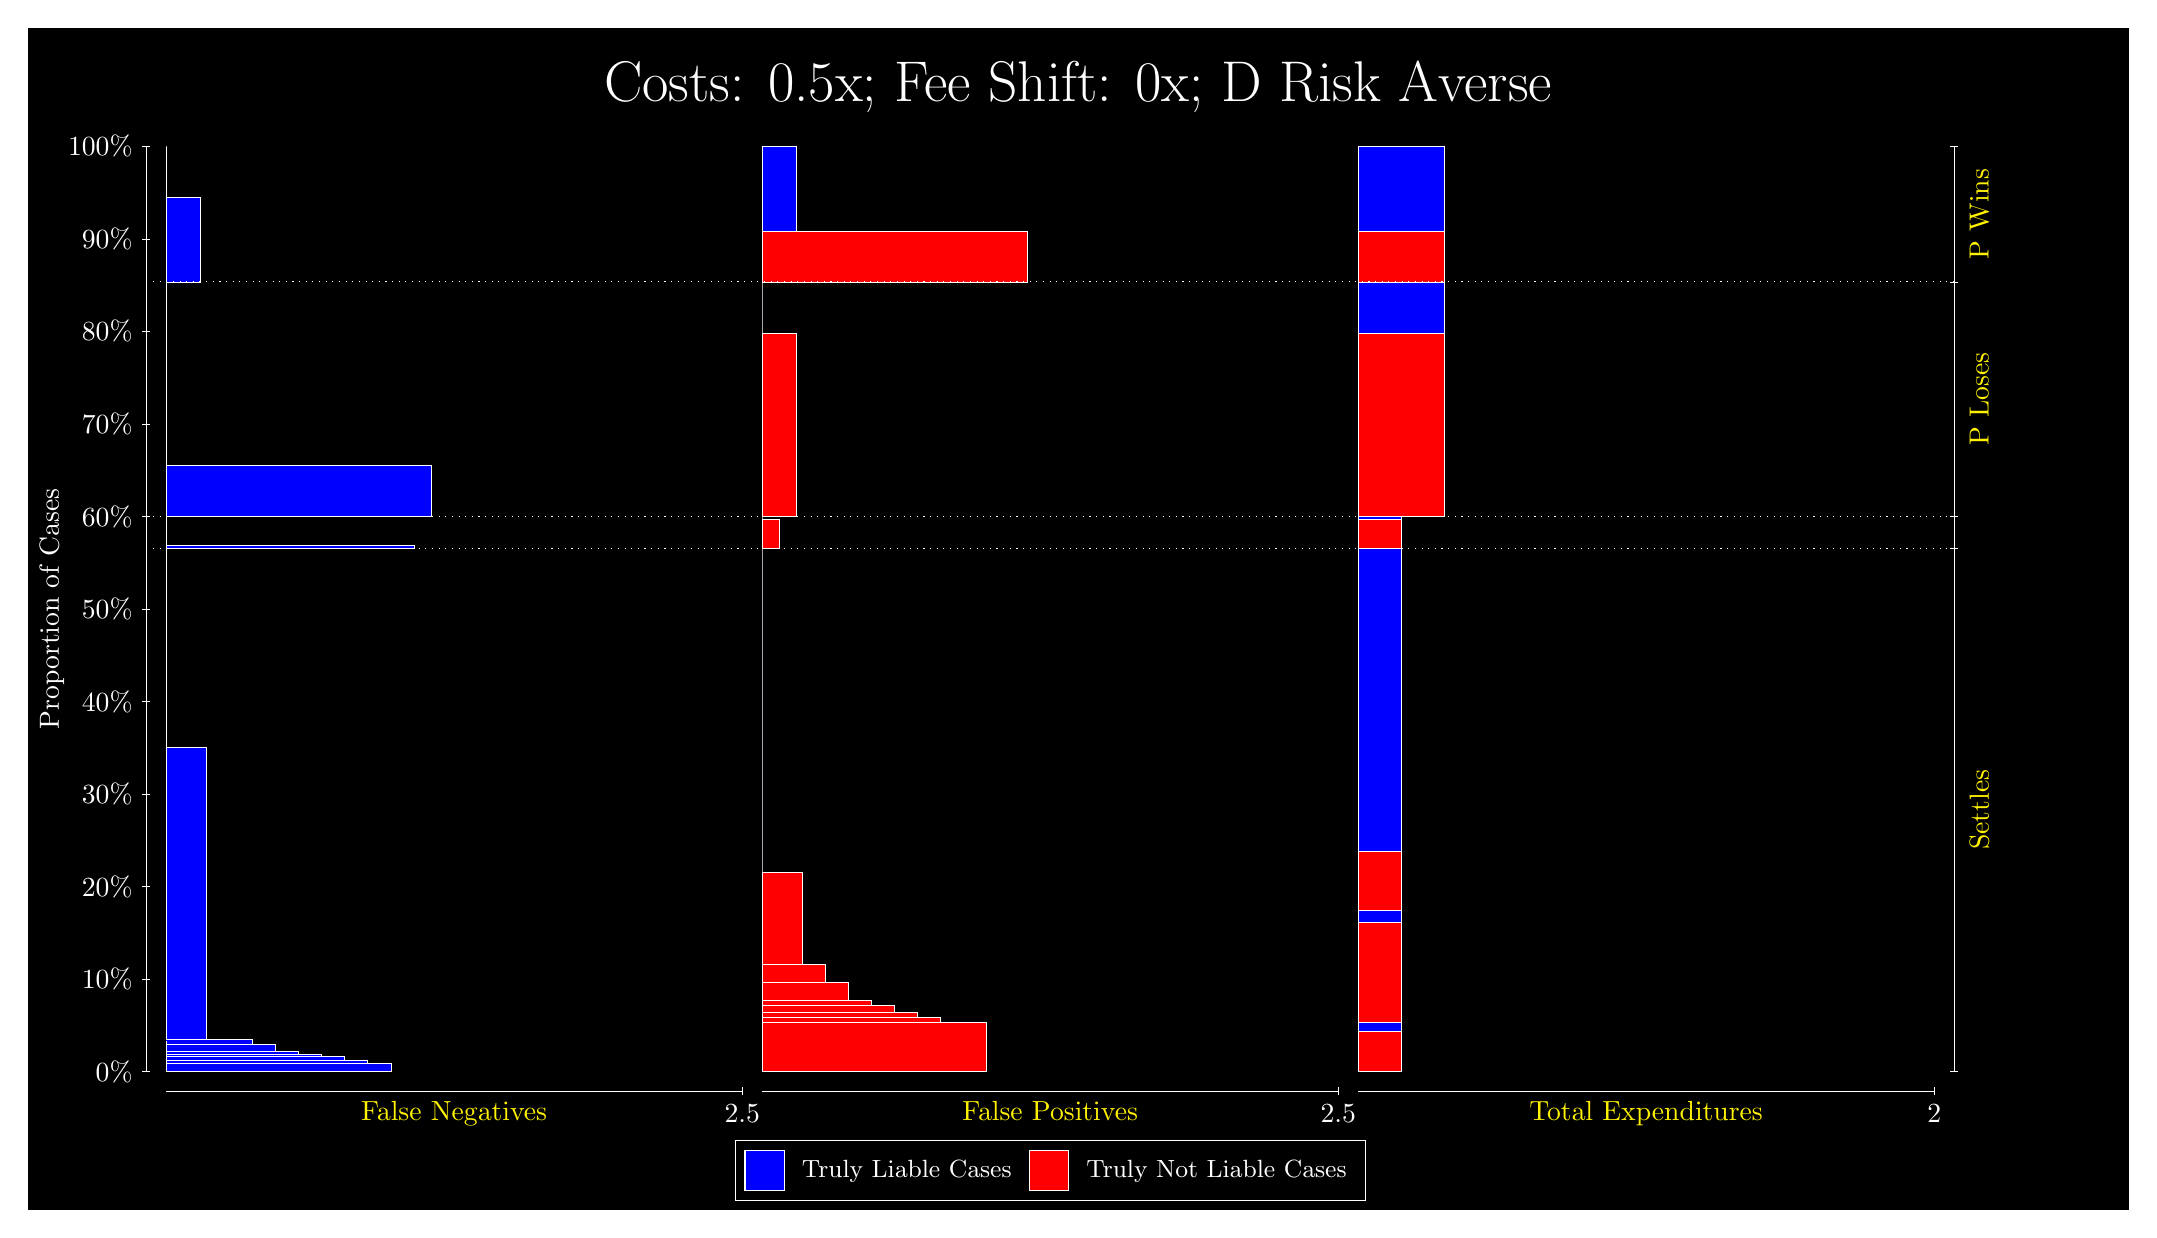
\begin{tikzpicture}
\draw[fill=black] (0,0) rectangle (26.667,15);
\draw[text=white] (0,13.5) rectangle (26.667,15) node[midway] {\huge Costs: 0.5x; Fee Shift: 0x; D Risk Averse};
\draw[white, very thin] (1.5,1.75) -- (1.5,13.5);
\node[rotate=90, text=white, anchor=center] at (0.3, 7.625) {Proportion of Cases};
\draw[white, very thin] (1.45,1.75) -- (1.55,1.75);
\node[text=white, anchor=east] at (1.45, 1.75) {0\%};
\draw[white, very thin] (1.45,2.925) -- (1.55,2.925);
\node[text=white, anchor=east] at (1.45, 2.925) {10\%};
\draw[white, very thin] (1.45,4.1) -- (1.55,4.1);
\node[text=white, anchor=east] at (1.45, 4.1) {20\%};
\draw[white, very thin] (1.45,5.275) -- (1.55,5.275);
\node[text=white, anchor=east] at (1.45, 5.275) {30\%};
\draw[white, very thin] (1.45,6.45) -- (1.55,6.45);
\node[text=white, anchor=east] at (1.45, 6.45) {40\%};
\draw[white, very thin] (1.45,7.625) -- (1.55,7.625);
\node[text=white, anchor=east] at (1.45, 7.625) {50\%};
\draw[white, very thin] (1.45,8.8) -- (1.55,8.8);
\node[text=white, anchor=east] at (1.45, 8.8) {60\%};
\draw[white, very thin] (1.45,9.975) -- (1.55,9.975);
\node[text=white, anchor=east] at (1.45, 9.975) {70\%};
\draw[white, very thin] (1.45,11.15) -- (1.55,11.15);
\node[text=white, anchor=east] at (1.45, 11.15) {80\%};
\draw[white, very thin] (1.45,12.325) -- (1.55,12.325);
\node[text=white, anchor=east] at (1.45, 12.325) {90\%};
\draw[white, very thin] (1.45,13.5) -- (1.55,13.5);
\node[text=white, anchor=east] at (1.45, 13.5) {100\%};

\draw[white, very thin] (24.457,1.75) -- (24.457,13.5);
\draw[white, very thin] (24.407,1.75) -- (24.507,1.75);
\node[anchor=west] at (24.407, 1.75) {};
\draw[white, very thin] (24.407,8.3973) -- (24.507,8.3973);
\node[anchor=west] at (24.407, 8.3973) {};
\draw[white, very thin] (24.407,8.801) -- (24.507,8.801);
\node[anchor=west] at (24.407, 8.801) {};
\draw[white, very thin] (24.407,11.778) -- (24.507,11.778);
\node[anchor=west] at (24.407, 11.778) {};
\draw[white, very thin] (24.407,13.5) -- (24.507,13.5);
\node[anchor=west] at (24.407, 13.5) {};

\draw[white, very thin, fill=blue] (1.75,1.75) rectangle (4.6044,1.8564);
\draw[white, very thin, fill=blue] (1.75,1.8564) rectangle (4.3116,1.8887);
\draw[white, very thin, fill=blue] (1.75,1.8887) rectangle (4.0188,1.9464);
\draw[white, very thin, fill=blue] (1.75,1.9464) rectangle (3.7261,1.9685);
\draw[white, very thin, fill=blue] (1.75,1.9685) rectangle (3.4333,2.0132);
\draw[white, very thin, fill=blue] (1.75,2.0132) rectangle (3.1406,2.0902);
\draw[white, very thin, fill=blue] (1.75,2.0902) rectangle (2.8478,2.1535);
\draw[white, very thin, fill=blue] (1.75,2.1535) rectangle (2.5551,2.1546);
\draw[white, very thin, fill=blue] (1.75,2.1546) rectangle (2.2623,5.862);
\draw[white, very thin, fill=red] (1.75,5.862) rectangle (1.75,8.3973);
\draw[white, very thin, fill=blue] (1.75,8.3973) rectangle (4.8971,8.4326);
\draw[white, very thin, fill=red] (1.75,8.4326) rectangle (1.75,8.801);
\draw[white, very thin, fill=blue] (1.75,8.801) rectangle (5.1167,9.4525);
\draw[white, very thin, fill=red] (1.75,9.4525) rectangle (1.75,11.778);
\draw[white, very thin, fill=blue] (1.75,11.778) rectangle (2.1891,12.854);
\draw[white, very thin, fill=red] (1.75,12.854) rectangle (1.75,13.5);
\draw[white, very thin, fill=red] (9.3189,1.75) rectangle (12.173,2.3797);
\draw[white, very thin, fill=red] (9.3189,2.3797) rectangle (11.88,2.3818);
\draw[white, very thin, fill=red] (9.3189,2.3818) rectangle (11.588,2.4352);
\draw[white, very thin, fill=red] (9.3189,2.4352) rectangle (11.295,2.5036);
\draw[white, very thin, fill=red] (9.3189,2.5036) rectangle (11.002,2.596);
\draw[white, very thin, fill=red] (9.3189,2.596) rectangle (10.709,2.6504);
\draw[white, very thin, fill=red] (9.3189,2.6504) rectangle (10.417,2.8781);
\draw[white, very thin, fill=red] (9.3189,2.8781) rectangle (10.124,3.1073);
\draw[white, very thin, fill=red] (9.3189,3.1073) rectangle (9.8312,4.2853);
\draw[white, very thin, fill=blue] (9.3189,4.2853) rectangle (9.3189,8.3973);
\draw[white, very thin, fill=red] (9.3189,8.3973) rectangle (9.5384,8.7657);
\draw[white, very thin, fill=blue] (9.3189,8.7657) rectangle (9.3189,8.801);
\draw[white, very thin, fill=red] (9.3189,8.801) rectangle (9.758,11.127);
\draw[white, very thin, fill=blue] (9.3189,11.127) rectangle (9.3189,11.778);
\draw[white, very thin, fill=red] (9.3189,11.778) rectangle (12.686,12.424);
\draw[white, very thin, fill=blue] (9.3189,12.424) rectangle (9.758,13.5);
\draw[white, very thin, fill=red] (16.888,1.75) rectangle (17.437,2.2613);
\draw[white, very thin, fill=blue] (16.888,2.2613) rectangle (17.437,2.3735);
\draw[white, very thin, fill=red] (16.888,2.3735) rectangle (17.437,3.6438);
\draw[white, very thin, fill=blue] (16.888,3.6438) rectangle (17.437,3.7948);
\draw[white, very thin, fill=red] (16.888,3.7948) rectangle (17.437,4.5484);
\draw[white, very thin, fill=blue] (16.888,4.5484) rectangle (17.437,8.3973);
\draw[white, very thin, fill=red] (16.888,8.3973) rectangle (17.437,8.7657);
\draw[white, very thin, fill=blue] (16.888,8.7657) rectangle (17.437,8.801);
\draw[white, very thin, fill=red] (16.888,8.801) rectangle (17.986,11.127);
\draw[white, very thin, fill=blue] (16.888,11.127) rectangle (17.986,11.778);
\draw[white, very thin, fill=red] (16.888,11.778) rectangle (17.986,12.424);
\draw[white, very thin, fill=blue] (16.888,12.424) rectangle (17.986,13.5);
\draw[white, dotted] (1.5,8.3973) -- (24.457,8.3973);
\draw[white, dotted] (1.5,8.801) -- (24.457,8.801);
\draw[white, dotted] (1.5,11.778) -- (24.457,11.778);
\draw[white, very thin] (1.75,1.5) -- (9.0689,1.5);
\node[text=yellow, anchor=north] at (5.4094, 1.5) {False Negatives};
\draw[white, very thin] (9.0689,1.45) -- (9.0689,1.55);
\node[text=white, anchor=north] at (9.0689, 1.45) {2.5};

\draw[white, very thin] (9.3189,1.5) -- (16.638,1.5);
\node[text=yellow, anchor=north] at (12.978, 1.5) {False Positives};
\draw[white, very thin] (16.638,1.45) -- (16.638,1.55);
\node[text=white, anchor=north] at (16.638, 1.45) {2.5};

\draw[white, very thin] (16.888,1.5) -- (24.207,1.5);
\node[text=yellow, anchor=north] at (20.547, 1.5) {Total Expenditures};
\draw[white, very thin] (24.207,1.45) -- (24.207,1.55);
\node[text=white, anchor=north] at (24.207, 1.45) {2};

\node[text=yellow, centered, rotate=90] at (24.777, 5.0737) {Settles};

\node[text=yellow, centered, rotate=90] at (24.777, 10.29) {P Loses};
\node[text=yellow, centered, rotate=90] at (24.777, 12.639) {P Wins};

\draw (12.978300999999998,1.5) node[draw=none] (baseCoordinate) {};
\begin{scope}[align=center]
        \matrix[scale=0.5, draw=white, below=0.5cm of baseCoordinate, nodes={draw}, column sep=0.1cm]{
            \node[rectangle, draw, minimum width=0.5cm, minimum height=0.5cm, fill=blue] {}; &
            \node[draw=none, font=\small, text=white] (B) {Truly Liable Cases}; &
            \node[rectangle, draw, minimum width=0.5cm, minimum height=0.5cm, fill=red] {}; &
            \node[draw=none, font=\small, text=white] (B) {Truly Not Liable Cases}; \\
            };
\end{scope}

\end{tikzpicture}
\end{document}